\documentclass{report}

\usepackage{biblatex}
\usepackage{hyperref}
\usepackage{minted}
\usepackage[bottom]{footmisc}
\usepackage{amsmath}
\usepackage{mdframed}
\usepackage{enumitem}
\usepackage{subcaption}
\usepackage{graphicx}
\graphicspath{{images/}}

\usepackage{chngcntr}
\counterwithout{figure}{chapter}

% alterar codigo no 2.4 para ter o mesmo after que o 2.3
% alterar error handling
% adicionar exemplos 2.3

\setlength{\parskip}{\bigskipamount}

\begin{document}

\tableofcontents

\chapter{Introduction}

\section{Objectives}

\begin{enumerate}
	\item .
\end{enumerate}

\chapter{Sending money using locks}
This chapter will focus on modeling in CCS the following scenario (and variants of it):

Figure \ref{fig:problem1} represents a simplified diagram where three
participants use a \texttt{send€} action to represent an atomic transfer of money. This scenario does not include
locks, which can lead to deadlocks when improperly implemented.

\begin{figure}[htbp]
    \centering
    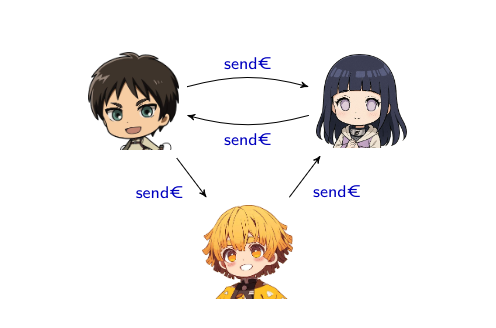
\includegraphics[width=0.75\textwidth]{problem1}
    \caption{Example scenario where different participants send money to each other}
    \label{fig:problem1}
\end{figure}
\section*{Exercise 1.1}
\addcontentsline{toc}{section}{Exercise 1.1}
Firstly, a simplified version of the original scenario is considered:

\begin{itemize}
	\item two participants always trying to send money to each other;
  \item the amount of money is ignored;
  \item \texttt{locks} are used in a naive way to force deadlocks to occurr.
\end{itemize}

The subsequent model of the scenario under consideration is formulated using CCS, with the consideration of two participants, Zenitsu and Hinata. Figure \ref{fig:naive} illustrates the respective LTS.

\begin{minted}{text}
let
  
  HinToZenDL = acqLockHin'.acqLockZen'.sendMoney.
               relLockZen'.relLockHin'.HinToZenDL;

  ZenToHinDL = acqLockZen'.acqLockHin'.sendMoney.
               relLockHin'.relLockZen'.ZenToHinDL;

  LockHinDL = acqLockHin.relLockHin.LockHinDL;

  LockZenDL = acqLockZen.relLockZen.LockZenDL;

in
  (HinToZenDL | ZenToHinDL | LockHinDL | LockZenDL) 
  \ {acqLockHin, acqLockZen, relLockHin, relLockZen}
\end{minted}

\begin{figure}[htbp]
    \centering
    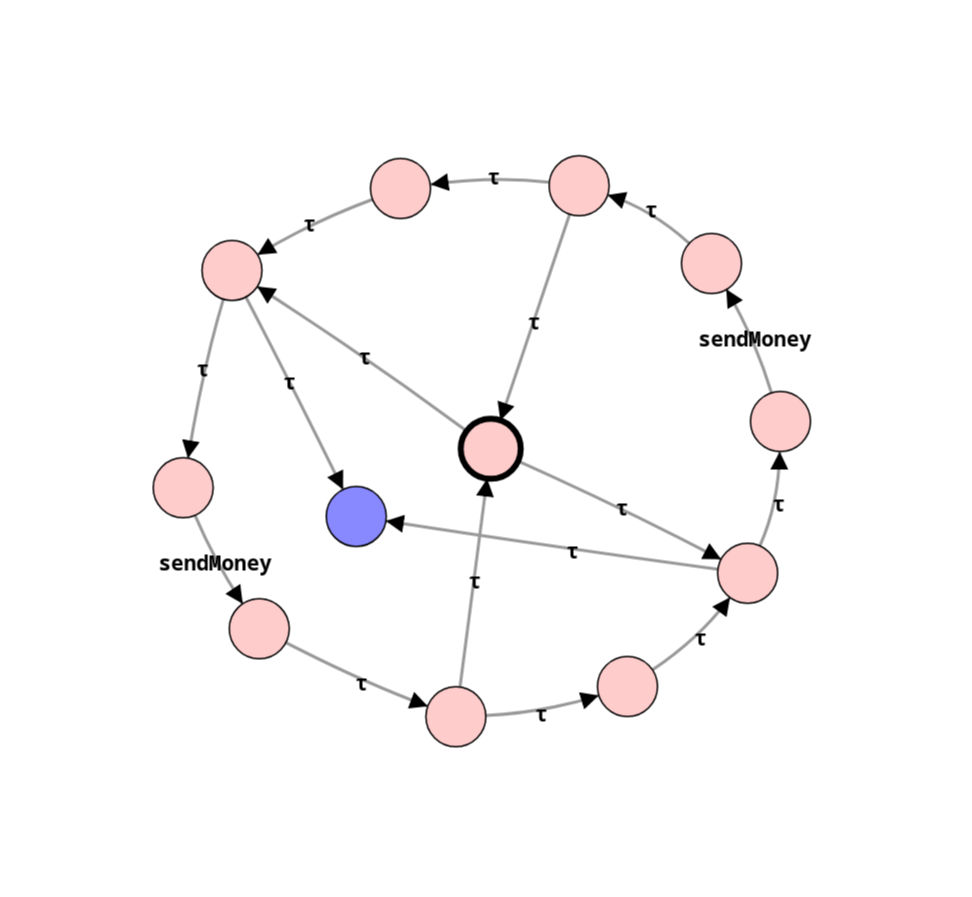
\includegraphics[width=0.75\textwidth]{naive}
    \caption{naive LTS}
    \label{fig:naive}
\end{figure}

\subsection*{Actions}
\addcontentsline{toc}{subsection}{Actions}

\begin{itemize}
    \item \texttt{acqLockHin}: acquisition of Hin's lock (sync);
    \item \texttt{relLockHin}: release of Hin's lock (sync);
    \item \texttt{acqLockZen}: acquisition of Zen's lock (sync); 
    \item \texttt{relLockZen}: release of Zen's lock (sync); 
    \item \texttt{sendMoney}: transfer of money.
\end{itemize}

It should be noted that each acquisition simulates Scala's \texttt{synchronized} construct behaviour in conjunction with its corresponding release. Moreover, it is not necessary to synchronise \texttt{sendMoney}, since the actions previously discussed ensure that this operation is performed atomically.

\subsection*{Processes}
\addcontentsline{toc}{subsection}{Processes}

\begin{itemize}
    \item \texttt{HinToZenDL}: representation of Hin trying to send money to Zen;
    \item \texttt{LockHinDL}: Hin's Lock associated with \texttt{HinToZenDL};
    \item \texttt{ZenToHinDL}: representation of Zen trying to send money to Hin; 
    \item \texttt{LockZenDL}: Zen's Lock associated with \texttt{ZenToHinDL}.
\end{itemize}

\section*{Exercise 1.2}
\addcontentsline{toc}{section}{Exercise 1.2}
The objective of this exercise is to adapt the model from the previous exercise to fix the deadlock. The approach used was to define a fixed order for lock acquisition. The idea is that Hin is always the first to acquire the lock, irrespective of his role, whether as the sender or the receiver.

\begin{minted}{text}
let
  
  HinZenSend = acqLockHin'.acqLockZen'.sendMoney.
               relLockZen'.relLockHin'.HinZenSend;

  LockHin = acqLockHin.relLockHin.LockHin;

  LockZen = acqLockZen.relLockZen.LockZen;

in
  (HinZenSend | HinZenSend | LockHin | LockZen) 
  \ {acqLockHin, acqLockZen, relLockHin, relLockZen}
\end{minted}

To date, two systems have been implemented in different ways to achieve the same desired outcome, namely the ability for two participants to transfer money to each other. These two systems are \texttt{not} weakly bisimilar, and we can prove it by simulating an attacker-defender game. The idea behind this is that the naive model exhibits a deadlock state, which the attacker can always access, irrespective of the defender's actions. This assertion is predicated on the notion that, at a certain point, the defender's capacity to replicate the attacker's actions becomes exhausted.

\subsection*{Weak Bisimilarity}
\addcontentsline{toc}{subsection}{Weak Bisimilarity}

\begin{mdframed}
\textbf{State 1} \\
\textbf{A:} strong $\tau$ (LTS1) \quad \textbf{D:} weak $\tau$ (LTS2)
\begin{align*}
\textit{LTS1:}\; & (\mathit{acqLockZen!}.\mathit{sendMoney}.\mathit{relLockZen!}.\mathit{relLockHin!}.\mathit{HinToZenDL} \\
                 & \mid \mathit{ZenToHinDL} \mid \mathit{relLockHin?}.\mathit{LockHinDL} \mid \mathit{LockZenDL}) \\
                 & \setminus \{\mathit{acqLockHin}, \mathit{acqLockZen}, \mathit{relLockHin}, \mathit{relLockZen}\} \\[6pt]
\textit{LTS2:}\; & (\mathit{acqLockZen!}.\mathit{sendMoney}.\mathit{relLockHin!}.\mathit{relLockZen!}.\mathit{HinZenSend} \\
                 & \mid \mathit{HinZenSend} \mid \mathit{relLockHin?}.\mathit{LockHin} \mid \mathit{LockZen}) \\
                 & \setminus \{\mathit{acqLockHin}, \mathit{acqLockZen}, \mathit{relLockHin}, \mathit{relLockZen}\}
\end{align*}
\end{mdframed}

\begin{mdframed}
\textbf{State 2} \\
\textbf{A:} strong $\tau$ (LTS1) \quad \textbf{D:} weak $\tau$ (LTS2)
\begin{align*}
\textit{LTS1:}\; & (\mathit{acqLockZen!}.\mathit{sendMoney}.\mathit{relLockZen!}.\mathit{relLockHin!}.\mathit{HinToZenDL} \\
                 & \mid \mathit{acqLockHin!}.\mathit{sendMoney}.\mathit{relLockHin!}.\mathit{relLockZen!}.\mathit{ZenToHinDL} \\
                 & \mid \mathit{relLockHin?}.\mathit{LockHinDL} \mid \mathit{relLockZen?}.\mathit{LockZenDL}) \\
                 & \setminus \{\mathit{acqLockHin}, \mathit{acqLockZen}, \mathit{relLockHin}, \mathit{relLockZen}\} \\[6pt]
\textit{LTS2:}\; & (\mathit{sendMoney}.\mathit{relLockHin!}.\mathit{relLockZen!}.\mathit{HinZenSend} \\
                 & \mid \mathit{HinZenSend} \mid \mathit{relLockHin?}.\mathit{LockHin} \mid \mathit{relLockZen?}.\mathit{LockZen}) \\
                 & \setminus \{\mathit{acqLockHin}, \mathit{acqLockZen}, \mathit{relLockHin}, \mathit{relLockZen}\}
\end{align*}
\end{mdframed}

\begin{mdframed}
\textbf{State 3} \\
\textbf{A:} strong $\mathit{sendMoney}$ (LTS2) \quad \textbf{D:} Impossible (LTS1)
\begin{align*}
\textit{LTS1:}\; & \emptyset \\[6pt]
\textit{LTS2:}\; & (\mathit{relLockHin!}.\mathit{relLockZen!}.\mathit{HinZenSend} \\
                 & \mid \mathit{HinZenSend} \mid \mathit{relLockHin?}.\mathit{LockHin} \mid \mathit{relLockZen?}.\mathit{LockZen}) \\
                 & \setminus \{\mathit{acqLockHin}, \mathit{acqLockZen}, \mathit{relLockHin}, \mathit{relLockZen}\}
\end{align*}
\end{mdframed}

\noindent The defender was unable to replicate the action of the attacker.  Consequently, we retrace the defender's actions to the previous state where alternative responses were possible (i.e.\ State 2).

\begin{mdframed}
\textbf{State 4} \\
\textbf{A:} strong $\tau$ (LTS1) \quad \textbf{D:} weak $\tau$ (LTS2)
\begin{align*}
\textit{LTS1:}\; & (\mathit{acqLockZen!}.\mathit{sendMoney}.\mathit{relLockZen!}.\mathit{relLockHin!}.\mathit{HinToZenDL} \\
                 & \mid \mathit{acqLockHin!}.\mathit{sendMoney}.\mathit{relLockHin!}.\mathit{relLockZen!}.\mathit{ZenToHinDL} \\
                 & \mid \mathit{relLockHin?}.\mathit{LockHinDL} \mid \mathit{relLockZen?}.\mathit{LockZenDL}) \\
                 & \setminus \{\mathit{acqLockHin}, \mathit{acqLockZen}, \mathit{relLockHin}, \mathit{relLockZen}\} \\[6pt]
\textit{LTS2:}\; & (\mathit{acqLockZen!}.\mathit{sendMoney}.\mathit{relLockHin!}.\mathit{relLockZen!}.\mathit{HinZenSend} \\
                 & \mid \mathit{HinZenSend} \mid \mathit{relLockHin?}.\mathit{LockHin} \mid \mathit{LockZen}) \\
                 & \setminus \{\mathit{acqLockHin}, \mathit{acqLockZen}, \mathit{relLockHin}, \mathit{relLockZen}\}
\end{align*}
\end{mdframed}

\begin{mdframed}
\textbf{State 5} \\
\textbf{A:} strong $\tau$ (LTS2) \quad \textbf{D:} weak $\tau$ (LTS1)
\begin{align*}
\textit{LTS1:}\; & (\mathit{acqLockZen!}.\mathit{sendMoney}.\mathit{relLockZen!}.\mathit{relLockHin!}.\mathit{HinToZenDL} \\
                 & \mid \mathit{acqLockHin!}.\mathit{sendMoney}.\mathit{relLockHin!}.\mathit{relLockZen!}.\mathit{ZenToHinDL} \\
                 & \mid \mathit{relLockHin?}.\mathit{LockHinDL} \mid \mathit{relLockZen?}.\mathit{LockZenDL}) \\
                 & \setminus \{\mathit{acqLockHin}, \mathit{acqLockZen}, \mathit{relLockHin}, \mathit{relLockZen}\} \\[6pt]
\textit{LTS2:}\; & (\mathit{sendMoney}.\mathit{relLockHin!}.\mathit{relLockZen!}.\mathit{HinZenSend} \\
                 & \mid \mathit{HinZenSend} \mid \mathit{relLockHin?}.\mathit{LockHin} \mid \mathit{relLockZen?}.\mathit{LockZen}) \\
                 & \setminus \{\mathit{acqLockHin}, \mathit{acqLockZen}, \mathit{relLockHin}, \mathit{relLockZen}\}
\end{align*}
\end{mdframed}

\noindent This state identical to State 2, which implies that the defender loses the game.  Consequently, we retrace the defender's actions to the previous state where alternative responses were possible (i.e.\ State 1).

\begin{mdframed}
\textbf{State 6} \\
\textbf{A:} strong $\tau$ (LTS1) \quad \textbf{D:} weak $\tau$ (LTS2)
\begin{align*}
\textit{LTS1:}\; & (\mathit{acqLockZen!}.\mathit{sendMoney}.\mathit{relLockZen!}.\mathit{relLockHin!}.\mathit{HinToZenDL} \\
                 & \mid \mathit{ZenToHinDL} \mid \mathit{relLockHin?}.\mathit{LockHinDL} \mid \mathit{LockZenDL}) \\
                 & \setminus \{\mathit{acqLockHin}, \mathit{acqLockZen}, \mathit{relLockHin}, \mathit{relLockZen}\} \\[6pt]
\textit{LTS2:}\; & (\mathit{HinZenSend} \mid \mathit{HinZenSend} \mid \mathit{LockHin} \mid \mathit{LockZen}) \\
                 & \setminus \{\mathit{acqLockHin}, \mathit{acqLockZen}, \mathit{relLockHin}, \mathit{relLockZen}\}
\end{align*}
\end{mdframed}

\begin{mdframed}
\textbf{State 7} \\
\textbf{A:} strong $\tau$ (LTS1) \quad \textbf{D:} weak $\tau$ (LTS2)
\begin{align*}
\textit{LTS1:}\; & (\mathit{acqLockZen!}.\mathit{sendMoney}.\mathit{relLockZen!}.\mathit{relLockHin!}.\mathit{HinToZenDL} \\
                 & \mid \mathit{acqLockHin!}.\mathit{sendMoney}.\mathit{relLockHin!}.\mathit{relLockZen!}.\mathit{ZenToHinDL} \\
                 & \mid \mathit{relLockHin?}.\mathit{LockHinDL} \mid \mathit{relLockZen?}.\mathit{LockZenDL}) \\
                 & \setminus \{\mathit{acqLockHin}, \mathit{acqLockZen}, \mathit{relLockHin}, \mathit{relLockZen}\} \\[6pt]
\textit{LTS2:}\; & (\mathit{acqLockZen!}.\mathit{sendMoney}.\mathit{relLockHin!}.\mathit{relLockZen!}.\mathit{HinZenSend} \\
                 & \mid \mathit{HinZenSend} \mid \mathit{relLockHin?}.\mathit{LockHin} \mid \mathit{LockZen}) \\
                 & \setminus \{\mathit{acqLockHin}, \mathit{acqLockZen}, \mathit{relLockHin}, \mathit{relLockZen}\}
\end{align*}
\end{mdframed}

\noindent This state identical to State 4, which implies that the defender loses the game.  Consequently, we retrace the defender's actions to the previous state where alternative responses were possible (i.e.\ State 7).

\begin{mdframed}
\textbf{State 8} \\
\textbf{A:} strong $\tau$ (LTS1) \quad \textbf{D:} weak $\tau$ (LTS2)
\begin{align*}
\textit{LTS1:}\; & (\mathit{acqLockZen!}.\mathit{sendMoney}.\mathit{relLockZen!}.\mathit{relLockHin!}.\mathit{HinToZenDL} \\
                 & \mid \mathit{acqLockHin!}.\mathit{sendMoney}.\mathit{relLockHin!}.\mathit{relLockZen!}.\mathit{ZenToHinDL} \\
                 & \mid \mathit{relLockHin?}.\mathit{LockHinDL} \mid \mathit{relLockZen?}.\mathit{LockZenDL}) \\
                 & \setminus \{\mathit{acqLockHin}, \mathit{acqLockZen}, \mathit{relLockHin}, \mathit{relLockZen}\} \\[6pt]
\textit{LTS2:}\; & (\mathit{HinZenSend} \mid \mathit{HinZenSend} \mid \mathit{LockHin} \mid \mathit{LockZen}) \\
                 & \setminus \{\mathit{acqLockHin}, \mathit{acqLockZen}, \mathit{relLockHin}, \mathit{relLockZen}\}
\end{align*}
\end{mdframed}

\begin{mdframed}
\textbf{State 9} \\
\textbf{A:} strong $\tau$ (LTS2) \quad \textbf{D:} weak $\tau$ (LTS1)
\begin{align*}
\textit{LTS1:}\; & (\mathit{acqLockZen!}.\mathit{sendMoney}.\mathit{relLockZen!}.\mathit{relLockHin!}.\mathit{HinToZenDL} \\
                 & \mid \mathit{acqLockHin!}.\mathit{sendMoney}.\mathit{relLockHin!}.\mathit{relLockZen!}.\mathit{ZenToHinDL} \\
                 & \mid \mathit{relLockHin?}.\mathit{LockHinDL} \mid \mathit{relLockZen?}.\mathit{LockZenDL}) \\
                 & \setminus \{\mathit{acqLockHin}, \mathit{acqLockZen}, \mathit{relLockHin}, \mathit{relLockZen}\} \\[6pt]
\textit{LTS2:}\; & (\mathit{acqLockZen!}.\mathit{sendMoney}.\mathit{relLockHin!}.\mathit{relLockZen!}.\mathit{HinZenSend} \\
                 & \mid \mathit{HinZenSend} \mid \mathit{relLockHin?}.\mathit{LockHin} \mid \mathit{LockZen}) \\
                 & \setminus \{\mathit{acqLockHin}, \mathit{acqLockZen}, \mathit{relLockHin}, \mathit{relLockZen}\}
\end{align*}
\end{mdframed}

\noindent This state identical to State 4, which implies that the defender loses the game. It would be possible to backtrack again by selecting the process that has not been altered, $\mathit{HinZenSend}$. Nevertheless, it is evident that the outcome would be the same.

\section*{Exercise 1.3}
\addcontentsline{toc}{section}{Exercise 1.3}
In this exercise, the scenario from Figure \ref{fig:problem1} is employed, utilising locks in a naive way (where deadlocks may occur). The approach adopted in this instance is equivalent to that utilised in Exercise 1.1, but for the full scenario.

\begin{minted}{text}
let
  HinToErenDL = acqLockHin'.acqLockEren'.sendMoney.
                relLockEren'.relLockHin'.HinToErenDL;

  ErenToHinDL = acqLockEren'.acqLockHin'.sendMoney.
                relLockHin'.relLockEren'.ErenToHinDL;

  ErenToZenDL = acqLockEren'.acqLockZen'.sendMoney.
                relLockZen'.relLockEren'.ErenToZenDL;
  
  ZenToHinDL = acqLockZen'.acqLockHin'.sendMoney.
               relLockHin'.relLockZen'.ZenToHinDL;

  LockHinDL = acqLockHin.relLockHin.LockHinDL;
  
  LockErenDL = acqLockEren.relLockEren.LockErenDL;
  
  LockZenDL = acqLockZen.relLockZen.LockZenDL;

in
  (HinToErenDL | ErenToHinDL | ErenToZenDL | ZenToHinDL
  | LockHinDL | LockErenDL | LockZenDL) 
  \ 
  {acqLockHin, acqLockZen, acqLockEren, relLockHin, 
  relLockZen, relLockEren}
\end{minted}

\section*{Exercise 1.4}
\addcontentsline{toc}{section}{Exercise 1.4}

The scenario is now being generalised through the implementation of value-passing CCS, with three equivalent participants who can always send messages to any other participant. Recall the exercise 1.2 where fixed order for lock acquisition was used in order not to have deadlocks. This exercise uses the same approach, where the participant with the lower identifier, must acquire the lock first.

\subsection*{FIrst approach}
\addcontentsline{toc}{subsection}{First approach}

As previously stated in Exercise 1.2, the fixed order for lock acquisition was utilised in order to prevent deadlocks. This approach employs the same methodology, where the participant with the lower identifier must acquire the lock first. However, given the the generalisation of the model, all locks communicate through the same channel. Thus, when a participant attempts to acquire a lock, the action may synchronise with any lock process rather than exclusively with the lock associated with the participant. If it happens that it does not synchronise with the participant's lock, the possibility of deadlock and inconsistency arising is increased.

\begin{minted}{text}
FromTo[x, y] := (when (x < y) acqLock!x.acqLock!y.sendMoney.
                relLock!y.relLock!x.FromTo[x, y]) 
                + 
                (when (x >= y) acqLock!y.acqLock!x.sendMoney.
                relLock!x.relLock!y.FromTo[x, y])

Lock[x] := acqLock?x.relLock?x.Lock[x]

(FromTo[1, 2] | FromTo[2, 1] | FromTo[1, 3] | FromTo[3, 1] | 
 FromTo[2, 3] | FromTo[3, 2] | Lock[1] | Lock[2] | Lock[3]) 
 \ {acqLock, relLock}
\end{minted}

\subsection*{Second approach}
\addcontentsline{toc}{subsection}{Second approach}

*****FALAR AQUI*****

\begin{minted}{text}
FromTo[x, y] := (when (x < y) acqLock!x.ackAcqLock?z : Int.
                (when (x == z) acqLock!y.ackAcqLock?z : Int.
                (when (y == z) sendMoney.relLock!y.ackRelLock?z : Int.
                (when (y == z) relLock!x.ackRelLock?z : Int.
                (when (x == z) FromTo[x, y]))))) 
                + 
                (when (x >= y) acqLock!y.ackAcqLock?z : Int.
                (when (y == z) acqLock!x.ackAcqLock?z : Int.
                (when (x == z) sendMoney.relLock!x.ackRelLock?z : Int.
                (when (x == z) relLock!y.ackRelLock?z : Int.
                (when (y == z) FromTo[x, y])))))

Lock[x] := acqLock?z.(when (x == z) ackAcqLock!x.relLock?z.
           (when (x == z) ackRelLock!x.Lock[x]))

(FromTo[1, 2] | FromTo[2, 1] | FromTo[1, 3] | FromTo[3, 1] | 
 FromTo[2, 3] | FromTo[3, 2] | Lock[1] | Lock[2] | Lock[3]) 
 \ {acqLock, relLock}
\end{minted}

\chapter{Simulate dependent processes in a server}

This chapter will focus on adding support to the execution of simples instructions in a working skeleton server, following some requirements as listed below:

\begin{enumerate}
	\item the pending instructions should be managed by a thread pool with a fixed number of threads;
  \item the code that is executed (concurrently) when receiving a request should be as small as possible;
  \item if an instruction is ready to execute and there is an unused thread, the instruction should be
executed as soon as possible;
  \item shared data structures should be used to model the state of the server;
  \item three different kinds of requests can be made to the server:
    \begin{itemize}
      \item run a given block of instructions;
      \item ask for the state of the server;
      \item reset the state of the server. 
  \end{itemize}
  \item the result of the printing instruction should be stored by the server in its internal state (sent to
the client when requested).
\end{enumerate}

\section*{Exercise 2.1}
\addcontentsline{toc}{section}{Exercise 2.1}
It is important to note that the initial counter should count the quantity of requests that have been received. However it is not thread-safe (it may provide unexpected results).
As illustrated in Figure \ref{fig:unsafe}, this is an example of the kind of unanticipated outcomes that could be obtained. 

\begin{figure}[htbp]
\centering
\begin{subfigure}{.48\textwidth}
    \centering
    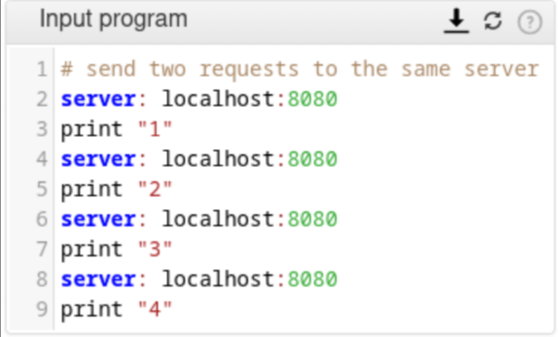
\includegraphics[width=1\textwidth]{unsafe1}
    \caption{Input}
    \label{fig:unsafe1}
\end{subfigure}
\begin{subfigure}{.48\textwidth}
    \centering
    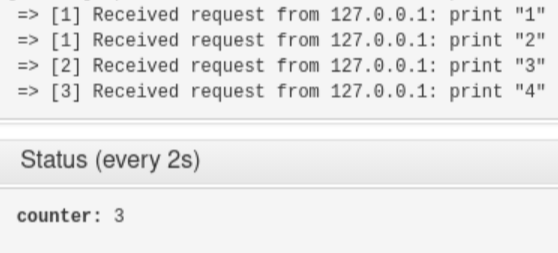
\includegraphics[width=1\textwidth]{unsafe2}
    \caption{Result}
    \label{fig:unsafe2}
\end{subfigure}
\caption{Example input where unexpected results are evident}
\label{fig:unsafe}
\end{figure}

It is to be expected that the counter will register four, given that four requests are being sent to the server. However, the result was not 4, but 3. This was due to the fact that the counter variable was not thread-safe. As demonstrated in Figure \ref{fig:drawio}, this sequence of events can be understood as a potential execution order that gave rise to the observed behaviour, where both threads write the value 1 to the counter. The solution to the issue lies in ensuring that the counter variable is made thread-safe. One method of achieving this is by changing its type from \texttt{Int} to \texttt{AtomicInteger}, and using its atomic operations (i.e. \texttt{incrementAndGet}).

\begin{figure}[htbp]
    \centering
    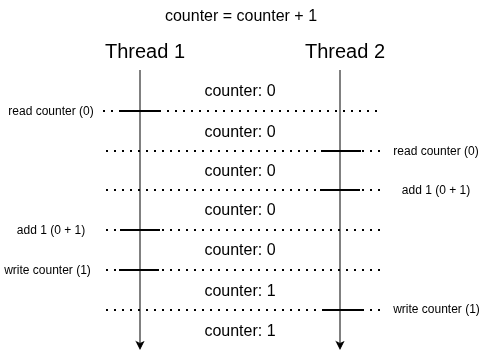
\includegraphics[width=0.75\textwidth]{drawio}
    \caption{Example of a bad sequence of events}
    \label{fig:drawio}
\end{figure}

\section*{Exercise 2.2}
\addcontentsline{toc}{section}{Exercise 2.2}

The next step is to extend the server to run the required instructions, ignoring for now the \texttt{after} clause. In order to achieve this, a thread pool with a predetermined number of threads (workers) was implemented so that the instructions could be executed concurrently. Listing \ref{lst:worker} presents the implementation of a worker. Lock-free programming was also employed for the purpose of storing the result of print instructions, by using an atomic variable, \texttt{AtomicReference[List[String]]}. 

\begin{listing}[htbp]
\caption{Worker implementation}
\label{lst:worker}
\begin{minted}{scala}
class Worker(
    tasks: mutable.Queue[(String, Option[Int])],
    content: AtomicReference[List[String]]
) extends Thread {
  setDaemon(true)
  def poll() = tasks.synchronized {
    while (tasks.isEmpty) tasks.wait()
    tasks.dequeue()
  }

  override def run() = while (true) {
    val (str, delayOpt) = poll()
    var delay = delayOpt match {
      case Some(d) => d
      case None    => 0
    }
    Thread.sleep(delay * 1000)

    val formatter = DateTimeFormatter.ofPattern("yyyy/MM/dd HH:mm:ss")
    val element =
      "[" ++ LocalDateTime.now().format(formatter) ++ "] " ++ str
    content.updateAndGet { old =>
      old :+ element
    }
  }
}

\end{minted}
\end{listing}

It is important to acknowledge that, if the shared structure was non-thread-safe, a comparable issue to that observed in exercise 2.1 with the counter would be encountered. In other words, one update could be overwritten by another, causing inconsistency. Figure \ref{fig:ex22} illustrates an example where such an inconsistency could occur. The first instruction could read the original value, [], and compute an updated version containing "hello1". However, prior to the rewriting of the update to the shared variable, it is possible that the second instruction would also read the same old value, [], and compute a different update containing "hello2". Consequently, the second write has the potential to overwrite the first one, resulting in the loss of one of the messages, and therefore fewer print messages. 

\begin{figure}[htbp]
    \centering
    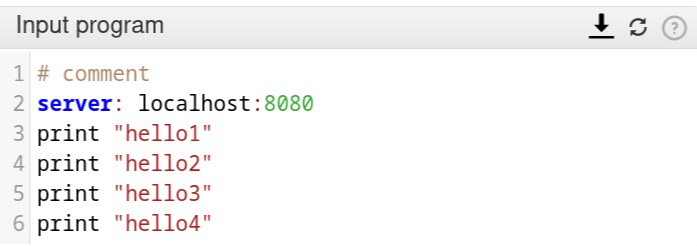
\includegraphics[width=0.75\textwidth]{ex22}
    \caption{Example input where unexpected results are evident}
    \label{fig:ex22}
\end{figure}

\section*{Exercise 2.3}
\addcontentsline{toc}{section}{Exercise 2.3}
Recall that the \texttt{after} clause was left unimplemented. In this exercise, three different approaches are examined and then compared with each other.

\subsection*{Bad implementation}
\addcontentsline{toc}{subsection}{Bad implementation}

The first idea was to create a data structure representing the topological ordering of the instruction dependencies. Therefore, two shared variables were introduced. The first of these variables was a map that mapped an instruction identifier to the instructions that depended on that key instruction to finish. The second variable was another map that also mapped an instruction identifier to an Int value representing the number of instructions that it was still contingent on. At first, all the instructions without any dependencies, are added to the queue. After the execution of an instruction, all instructions depending on it were updated by decreasing their current dependency count by one. Upon the occurrence of a count of zero for the designated instruction, the instruction was consequently added to the queue of tasks. 

However, given the utilisation of shared variables among threads, the identification of the instruction number as the sole identifier is not enough. Consequently, the atomic counter was utilised as a prefix. The chosen identifier is where the problem resides, as there is a possibility of the counter being reset and two different requests using the same counter on the instruction identifier.

\subsection*{Busy-waiting implementation}
\addcontentsline{toc}{subsection}{Busy-waiting implementation}

The initial concept was not entirely unsuccessful. However the proposal of distributing the maps amongst the threads was not a viable proposition. The solution to this issue was to implement the use of unique maps for each individual request. These maps were then provided as arguments to the threads, with the intention that they be updated atomically. The verification of whether an instruction possessed counter 0, a prerequisite for its processing, was conducted in a while loop in the runProcess() method. Whilst the proposed solution is indeed correct and consistent, it is important to note that busy waiting occurs. This is a process whereby the loop repetitively verifies a condition, thereby requiring processor power unnecessarily.

\subsection*{Non-busy-waiting implementation}
\addcontentsline{toc}{subsection}{Non-busy-waiting implementation}

The final approach, was built on top of the previous one, however, with only one difference. Instead of repetitively checking for 0, we only check if a counter is 0, when it is updated after the execution of an isntruction. 

\chapter{Conclusion}

% \printbibliography

\end{document}
